\section{Computation Complexity}
\label{sec:training}

We adopt the floating-point operations (FLOP) estimator for the Qwen2Model from verl~\cite{sheng2024hybridflow} to compute the FLOP cost of both the baseline model and our proposed method. The results are shown in Figure~\ref{fig:compute}. The baseline model exhibits an O($n^2$) complexity, while \method achieves an $O(n)$ complexity.

\begin{figure}[h]
    \centering
    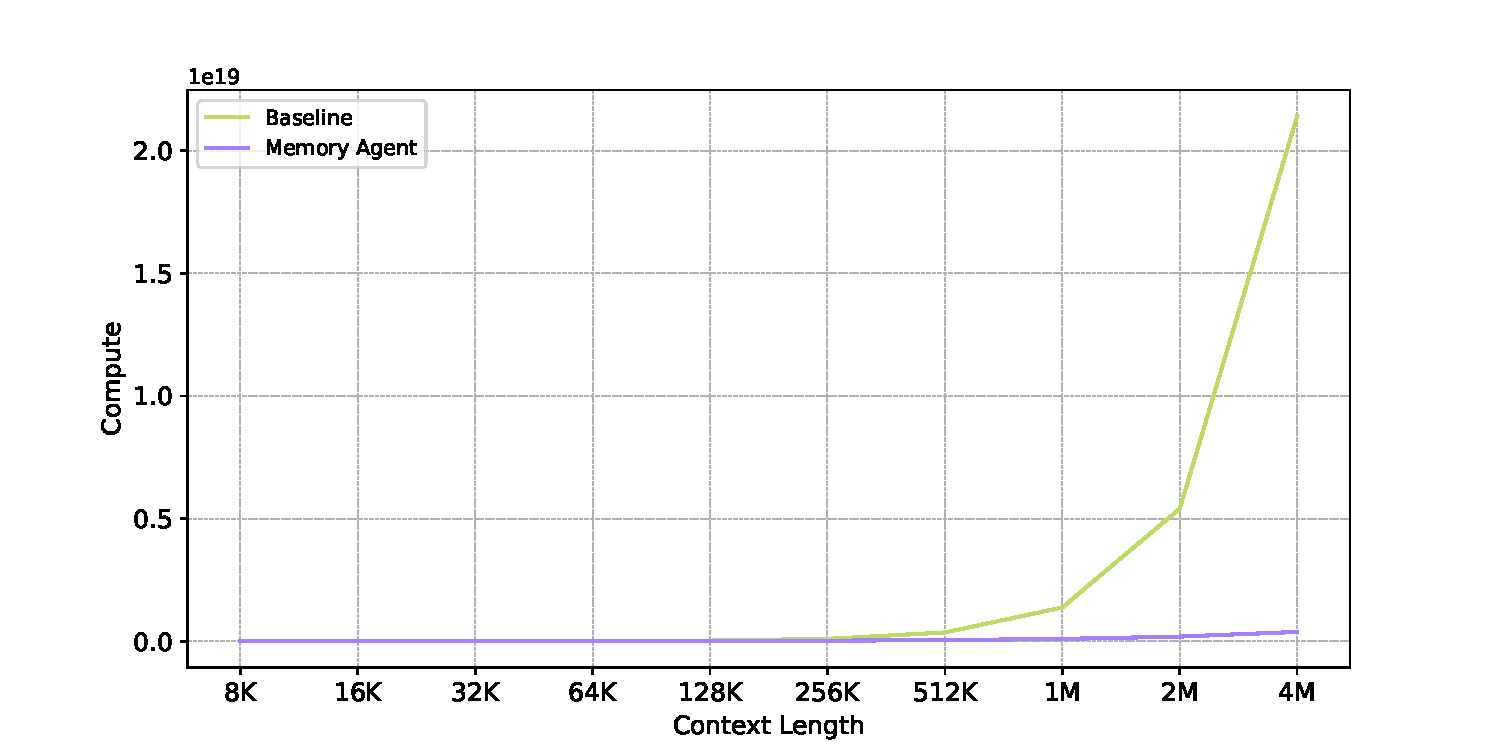
\includegraphics[width=0.9\linewidth]{figs/compute.pdf}
    \caption{Floating point operations across context lengths from 8K to 4M}
    \label{fig:compute}
\end{figure}

For the baseline model, the number of tokens required to process is $q + c + o$, where $q$ represents the length for the problem, $c$ is the context length and $o$ represents the output length.


For \method, total FLOP cost is the sum of the FLOPs from all stages. The detailed stages involved are as follows:

\begin{itemize}
\item Initializing: In the first stage, the model processes an input consisting of $q + 200 + o$, where  $200$ represents a constant added to prompt the model to follow the \method workflow.

\item Memory Updating: The number of repetitions is determined by $k=\lceil \frac{c}{N} \rceil$, where $c$ is the variable component of the input. Each repetition requires an input of length $q + 200 + N + o$.

\item Final Answering: The final stage processes an input of length $q + 100 + o$, which includes the accumulated output from the previous steps.
\end{itemize}

 We set $q=1024,o=1024,N=5000$ and $c$ is ranging from 8K to 4M to calculate the final result.

\section{Complete Out-Of-Domain Task Results}
\label{sec:OOD}

The RULER benchmark comprises tasks across four primary categories: retrieval, multi-hop tracing, aggregation, and question answering. Each task is designed to evaluate specific aspects of long-context modeling capability through automatically generated examples based on configurable input parameters that define sequence length and complexity. Within this constrained evaluation framework, task complexity can be conceptualized as a function of the number of target output tokens and the signal-to-noise ratio within the context.

The Needle-in-a-Haystack (NIAH) paradigm evaluates retrieval performance in long-context scenarios by inserting key-value pairs ("needles") into large distractor content ("haystack"). It includes four variants: Single NIAH, which requires retrieving a single needle; Multi-keys NIAH, which involves retrieving one needle amidst multiple distractors; Multi-values NIAH, where all values associated with a key must be extracted; and Multi-queries NIAH, which necessitates retrieving multiple needles with distinct keys. Variable Tracking (VT) tests multi-hop reasoning by tracking entity chains across extended sequences, while Frequent Words Extraction (FWE) challenges models to identify frequent words in power-law distributions, evaluating their ability to analyze word frequencies in linguistic data.


\subsection{Needle-in-a-Haystack (NIAH)}

\begin{figure}[htbp]
    \centering
    \begin{subfigure}{0.32\textwidth}
        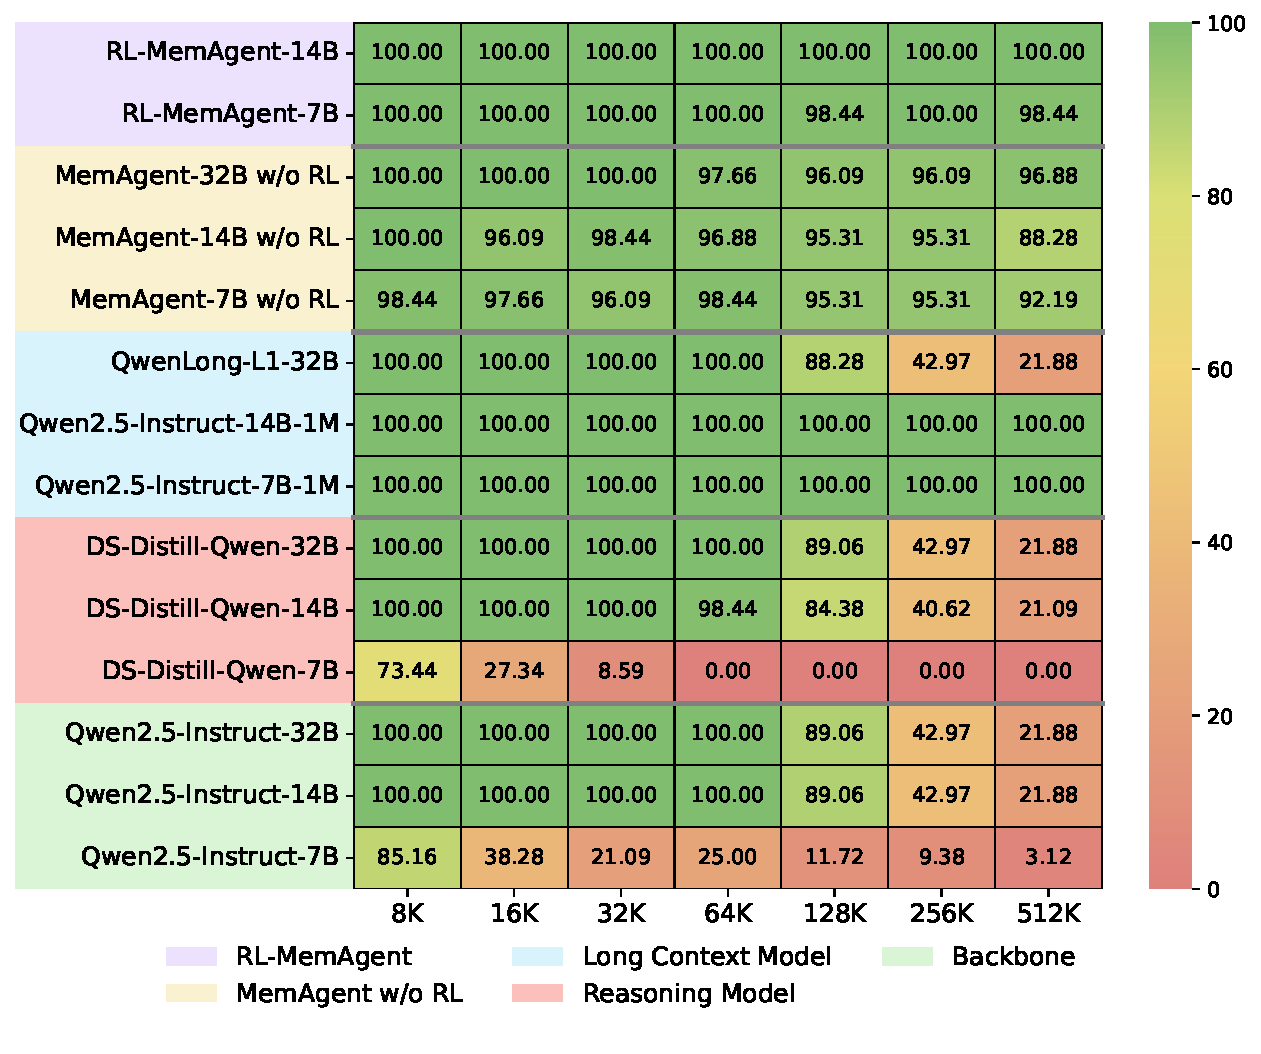
\includegraphics[width=\textwidth]{figs/niah_single_1.pdf}
        \caption{NIAH Single-key 1}
        \label{fig:niah-mk1}
    \end{subfigure}
    \hfill
    \begin{subfigure}{0.32\textwidth}
        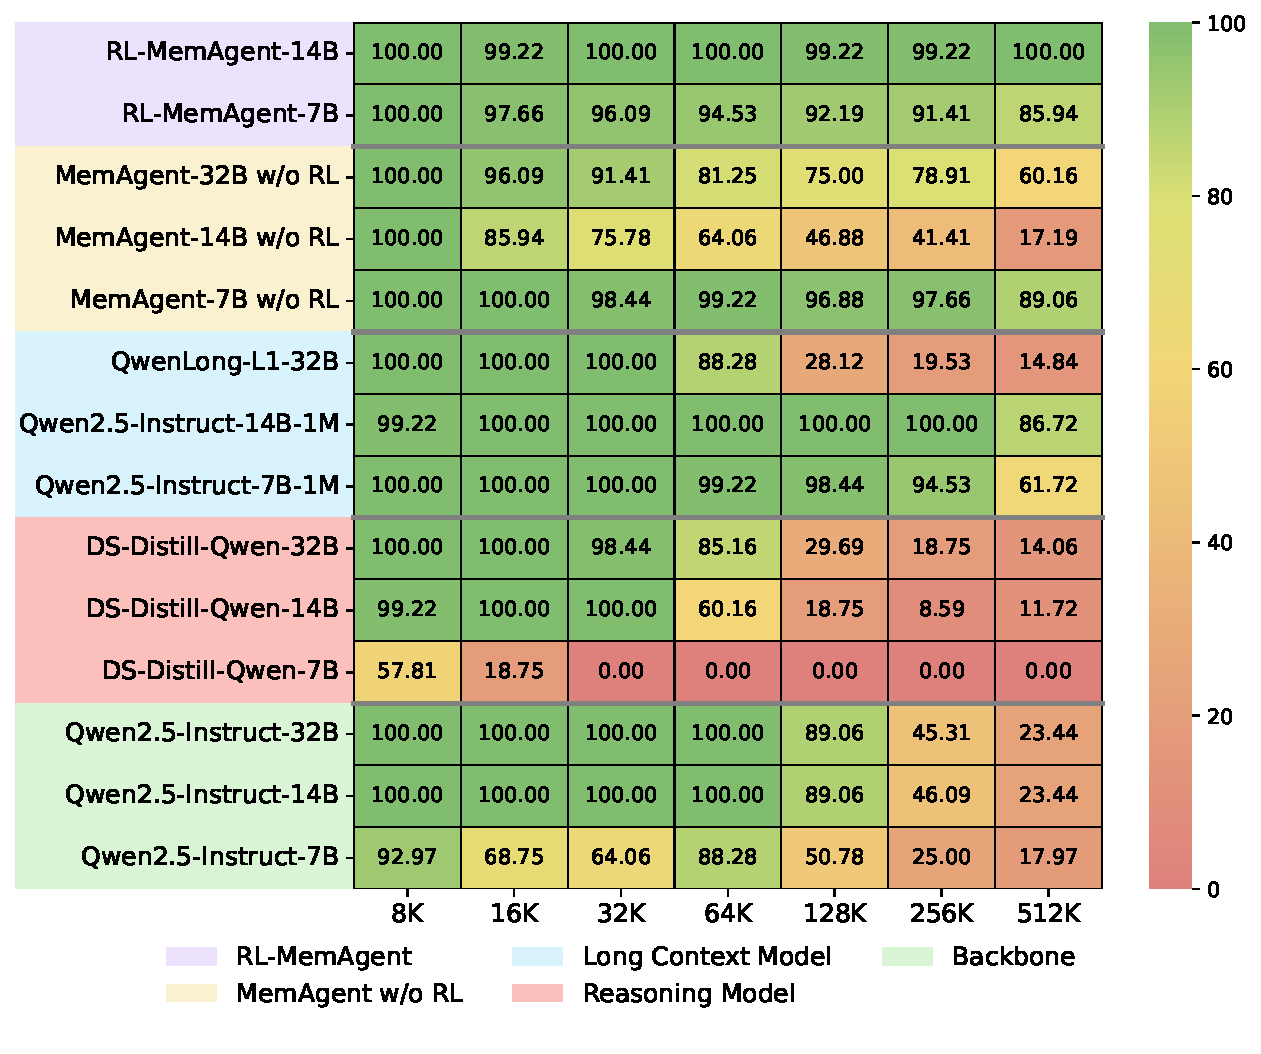
\includegraphics[width=\textwidth]{figs/niah_single_2.pdf}
        \caption{NIAH Single-key 2}
        \label{fig:niah-mk2}
    \end{subfigure}
    \hfill
    \begin{subfigure}{0.32\textwidth}
        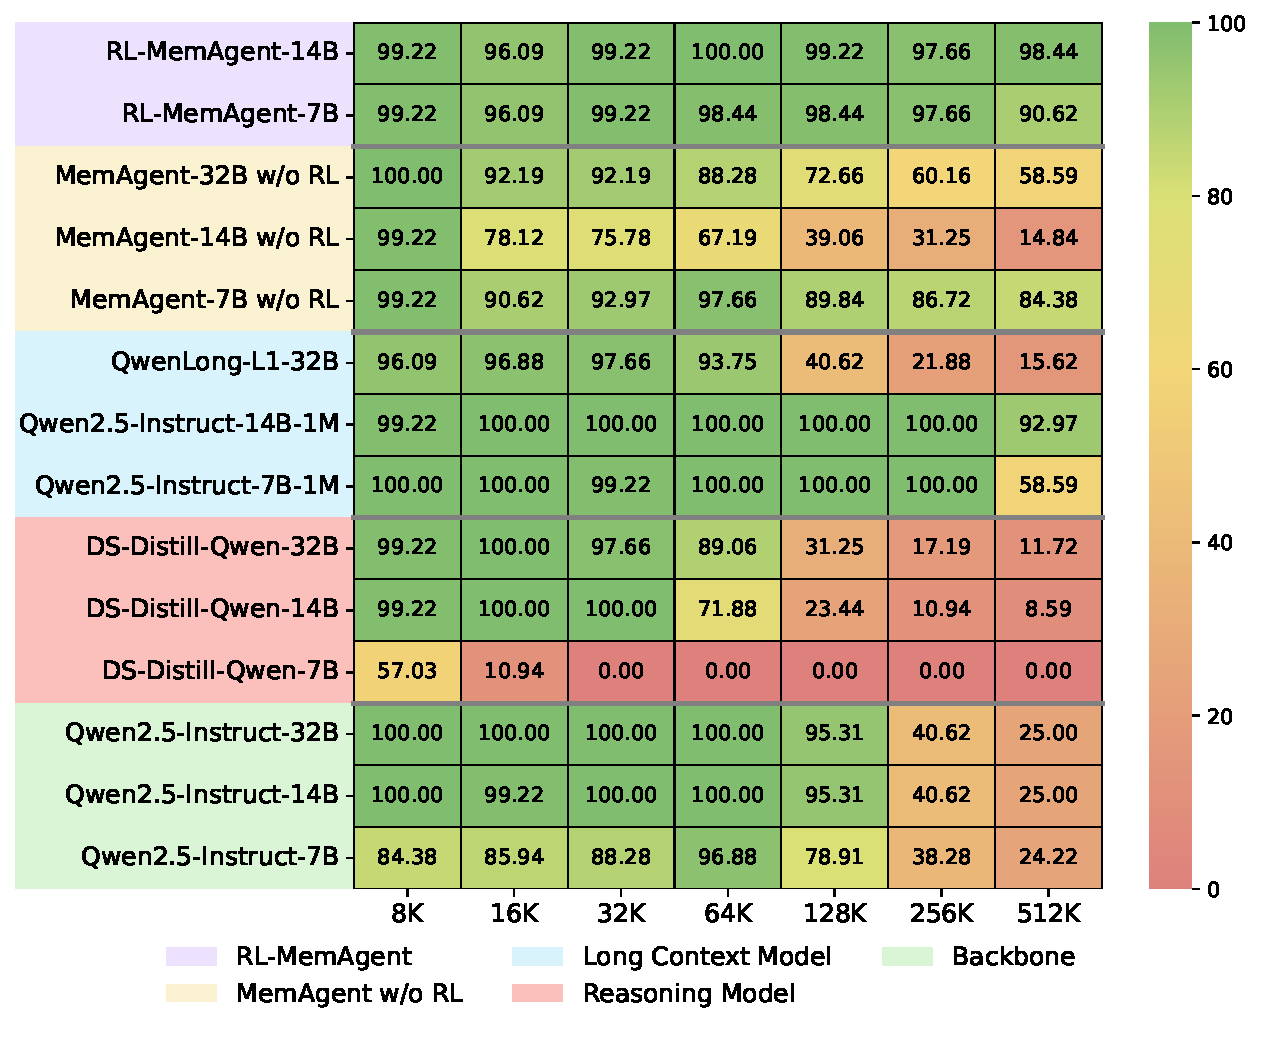
\includegraphics[width=\textwidth]{figs/niah_single_3.pdf}
        \caption{NIAH Single-key 3}
        \label{fig:niah-mk3}
    \end{subfigure}
    \caption{Performance on Single-keys NIAH tasks with increasing numbers of distractor needles. Tasks 1-3 represent different levels of difficulty with varying distractor densities.}
    \label{fig:niah-singlekey-all}
\end{figure}

\begin{figure}[h]
    \centering
    \begin{subfigure}{0.32\textwidth}
        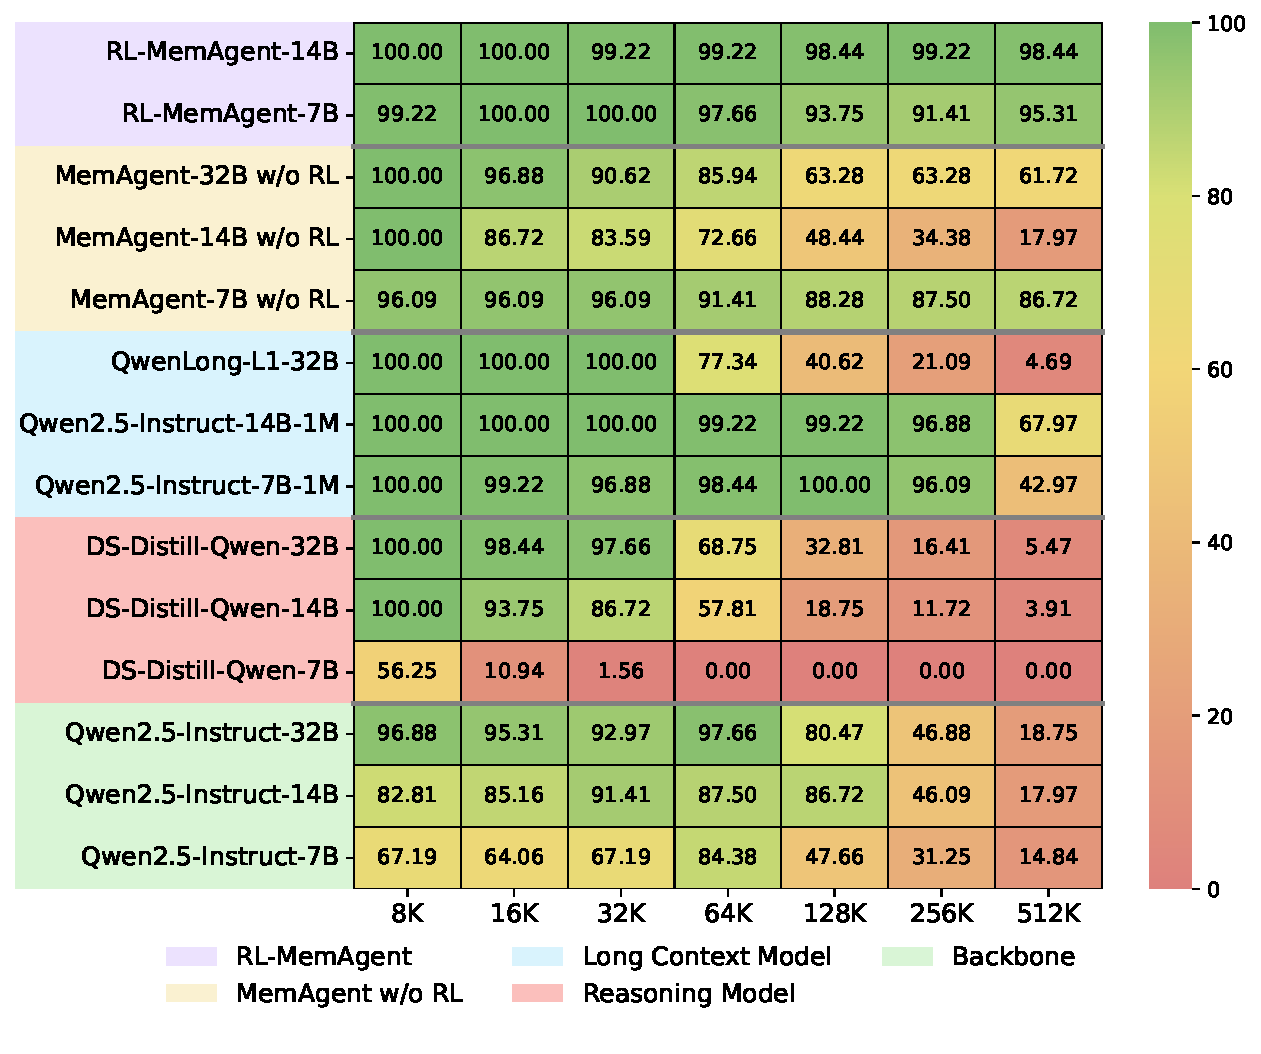
\includegraphics[width=\textwidth]{figs/niah_multikey_1.pdf}
        \caption{NIAH Multi-key 1}
        \label{fig:niah-mk1}
    \end{subfigure}
    \hfill
    \begin{subfigure}{0.32\textwidth}
        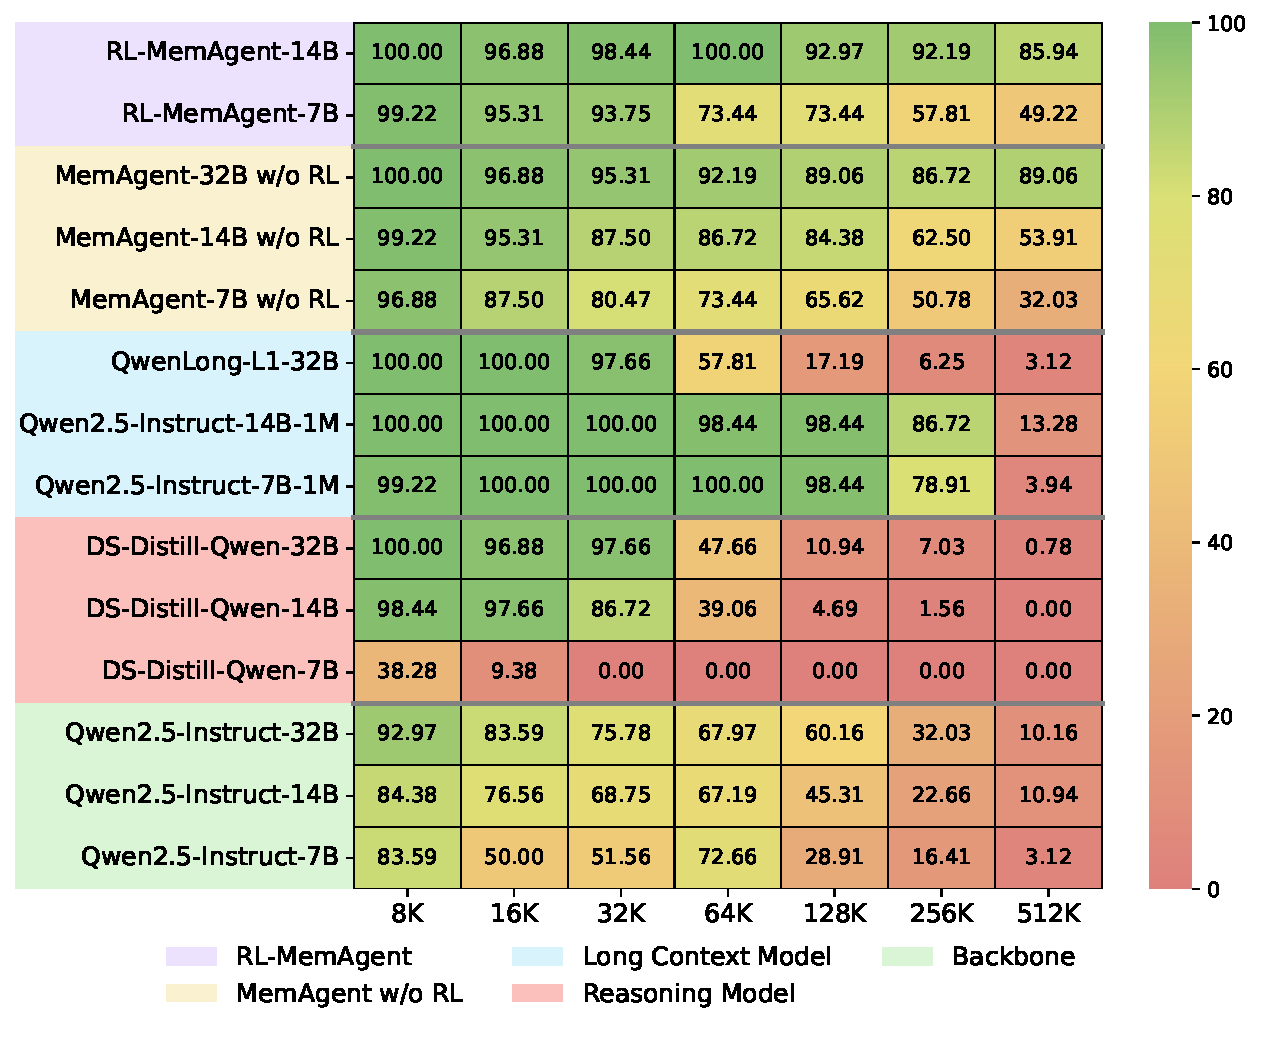
\includegraphics[width=\textwidth]{figs/niah_multikey_2.pdf}
        \caption{NIAH Multi-key 2}
        \label{fig:niah-mk2}
    \end{subfigure}
    \hfill
    \begin{subfigure}{0.32\textwidth}
        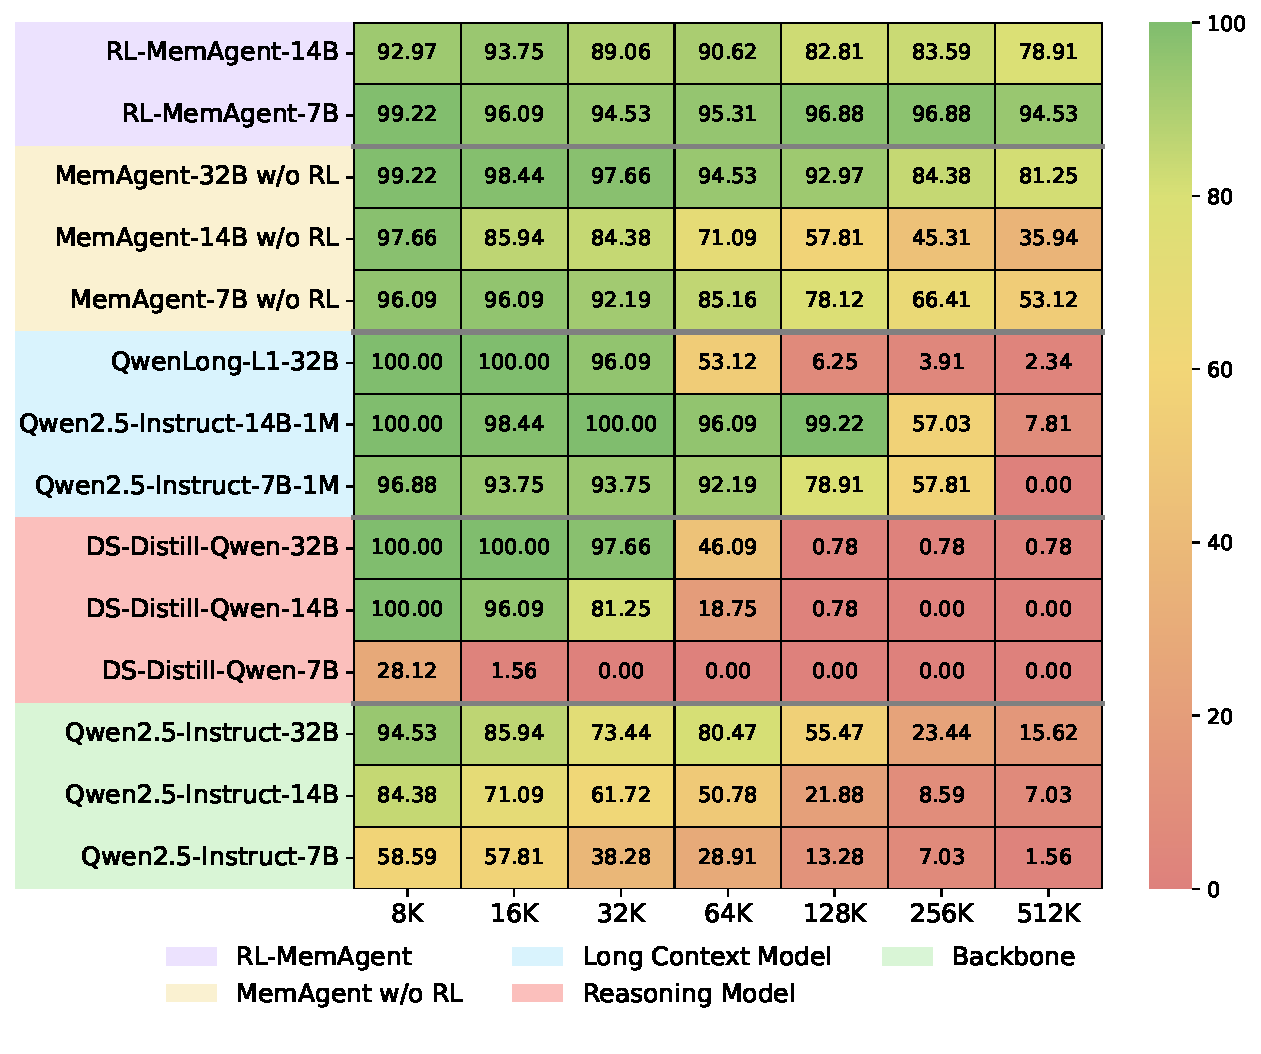
\includegraphics[width=\textwidth]{figs/niah_multikey_3.pdf}
        \caption{NIAH Multi-key 3}
        \label{fig:niah-mk3}
    \end{subfigure}
    \caption{Performance on Multi-keys NIAH tasks with increasing numbers of distractor needles. Tasks 1-3 represent different levels of difficulty with varying distractor densities.}
    \label{fig:niah-multikey-all}
\end{figure}

\begin{figure}[h]
    \centering
    \begin{subfigure}{0.48\textwidth}
        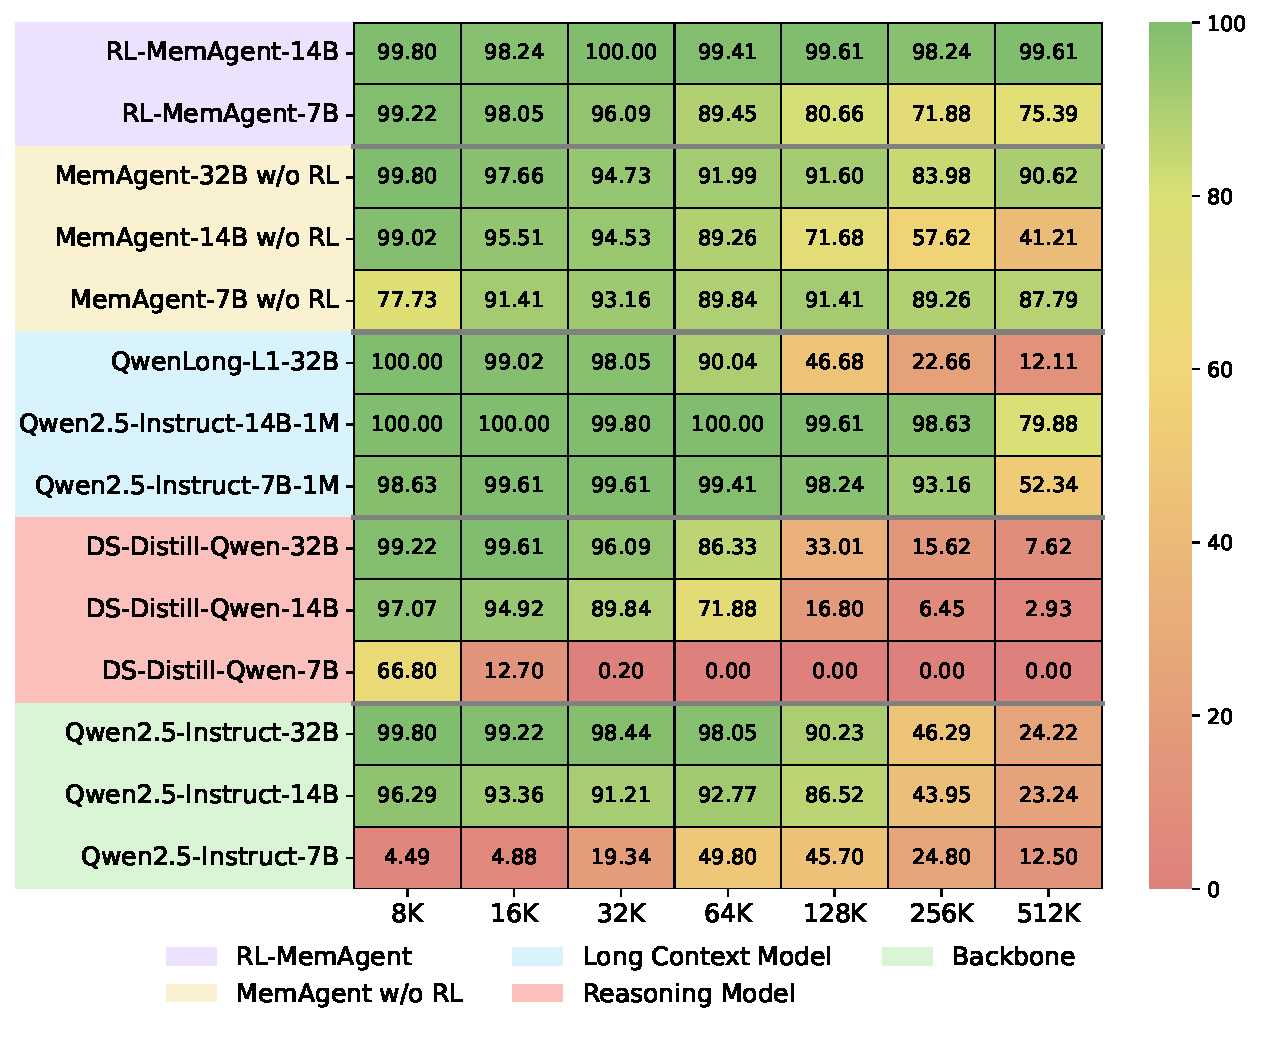
\includegraphics[width=\textwidth]{figs/niah_multiquery.pdf}
        \caption{NIAH Multi-query}
        \label{fig:niah-mq}
    \end{subfigure}
    \hfill
    \begin{subfigure}{0.48\textwidth}
        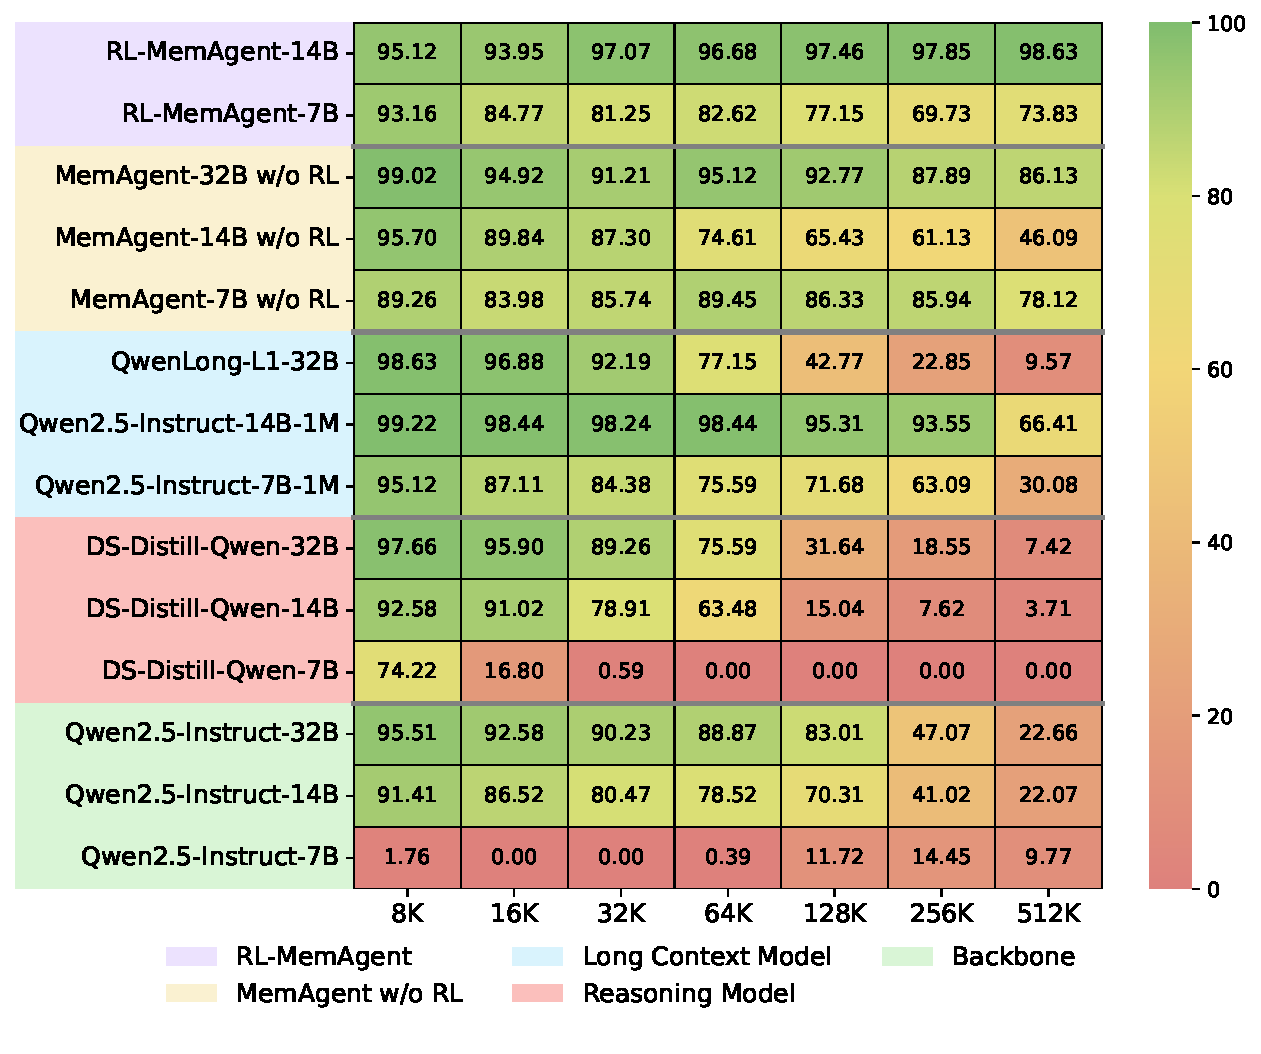
\includegraphics[width=\textwidth]{figs/niah_multivalue.pdf}
        \caption{NIAH Multi-value}
        \label{fig:niah-mv}
    \end{subfigure}
    \caption{Performance on advanced NIAH variants. (a) Multi-query task requiring retrieval of multiple distinct needles. (b) Multi-value task requiring extraction of all values sharing identical keys.}
    \label{fig:niah-advanced}
\end{figure}

\FloatBarrier

\subsection{Variable Tracking (VT) and Frequent Words Extraction (FWE)}


\begin{figure}[h]
    \centering
    \begin{subfigure}{0.48\textwidth}
        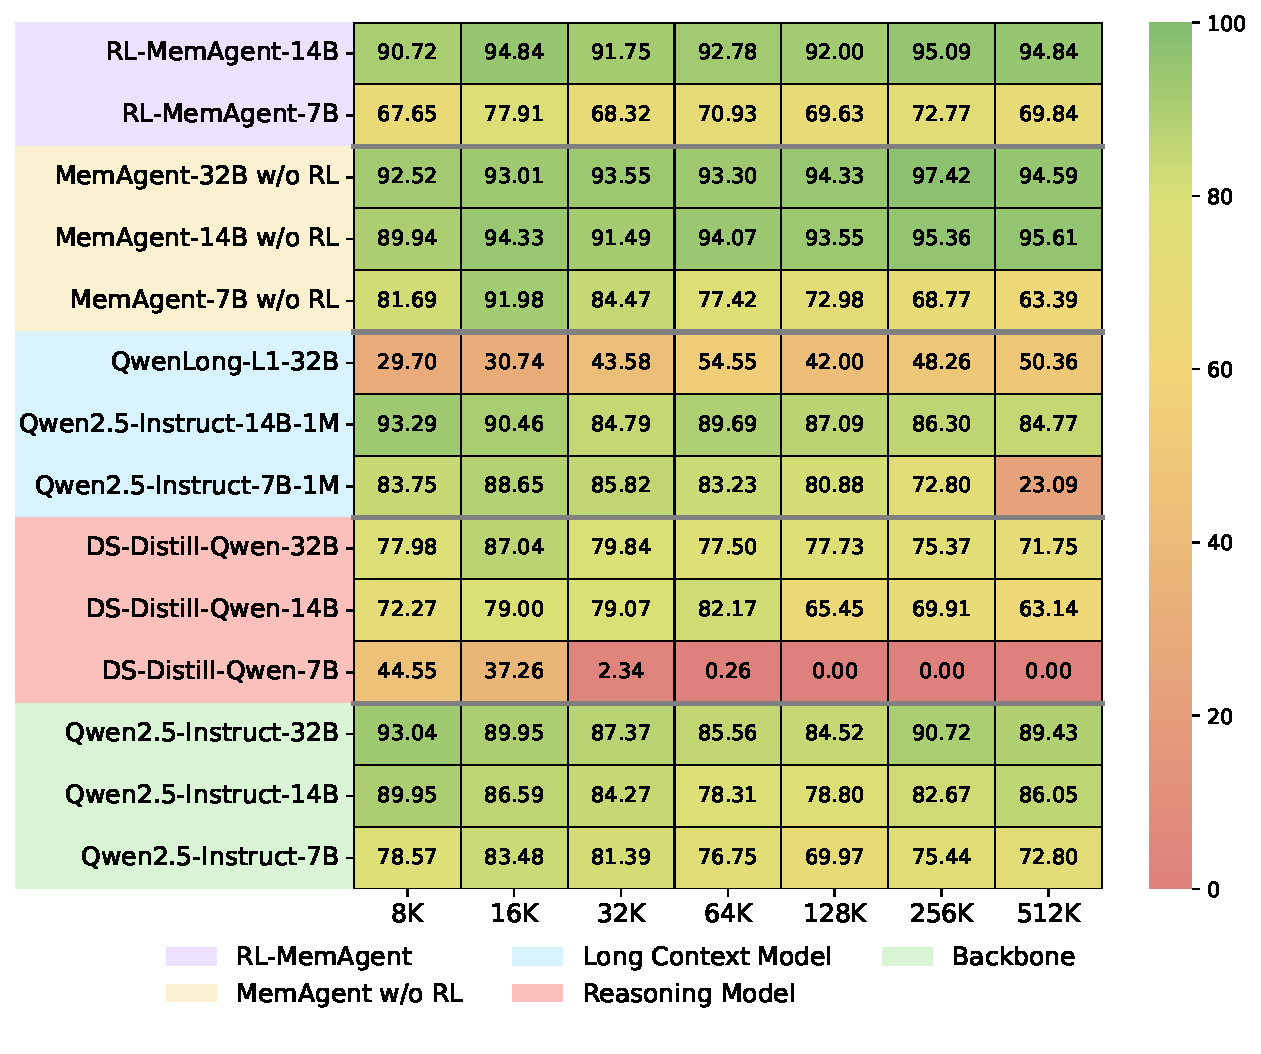
\includegraphics[width=\textwidth]{figs/fwe.pdf}
        \caption{Frequent Words Extraction}
        \label{fig:fwe}
    \end{subfigure}
    \hfill
    \begin{subfigure}{0.48\textwidth}
        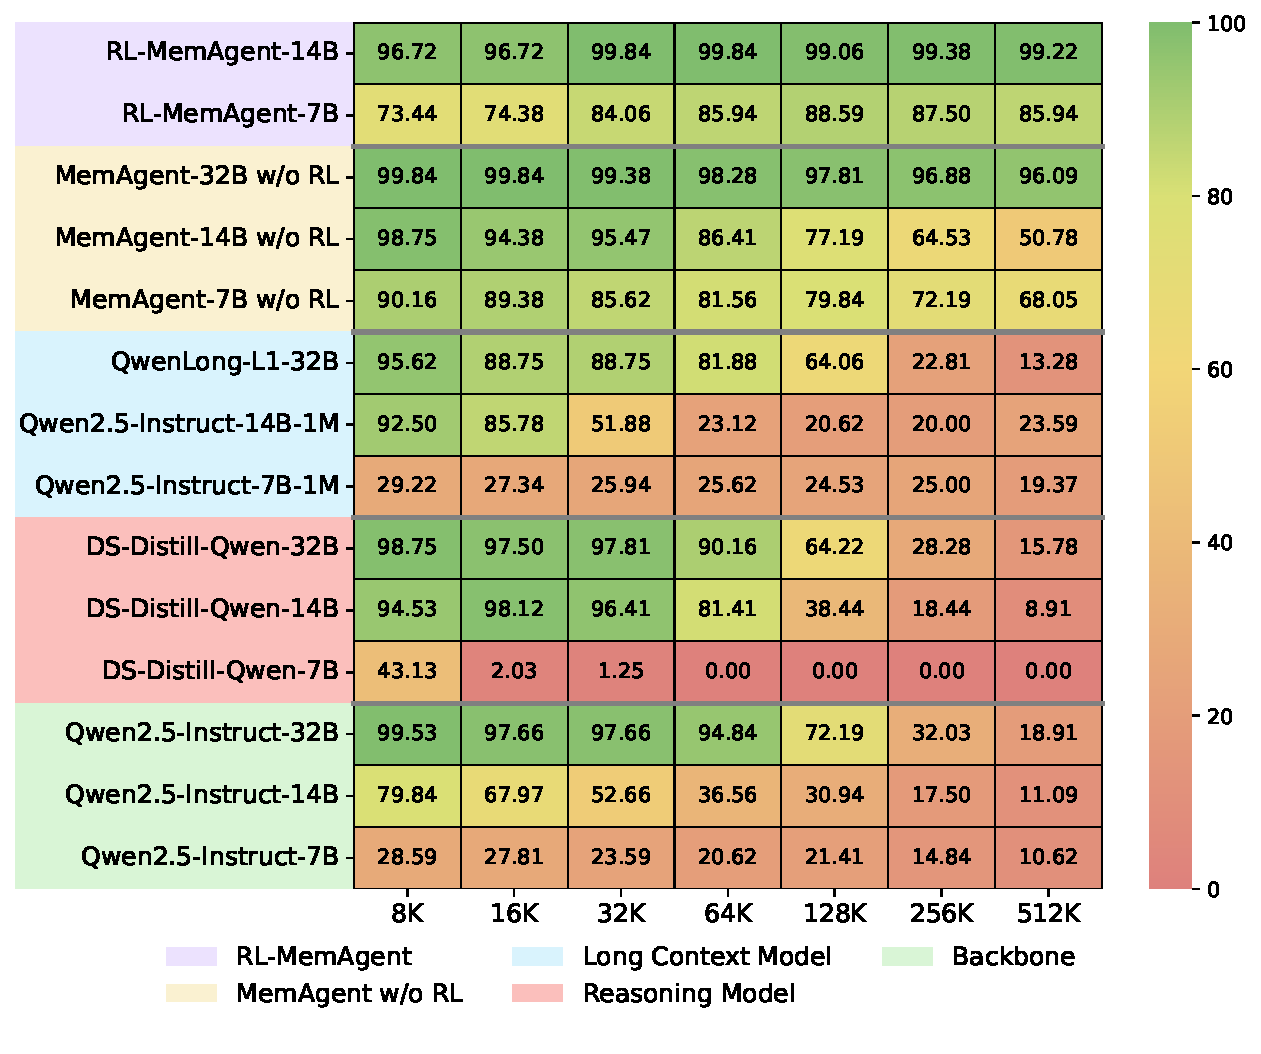
\includegraphics[width=\textwidth]{figs/vt.pdf}
        \caption{Variable Tracking}
        \label{fig:vt}
    \end{subfigure}
    \caption{Performance on frequent words extraction and variable tracking tasks.}
    \label{fig:non-retrieval}
\end{figure}